\section{Цель работы}
Для заданного объекта управления решить задачу адаптивного слежения.



\section{Теоретические сведения}
Рассматриваемый объект управления:
\begin{equation}
    \dot{x} = f(\theta_1, \theta_2, x) + u, \quad x(0), \\
\end{equation}
где $\theta_1$, $\theta_2$~--- неизвестные параметры.

Цель управления:
\begin{equation}
    \lim_{t \rightarrow \infty } \bigl( x_m(t) - x(t) \bigr) = \lim_{t \rightarrow \infty } \varepsilon(t) = 0,
\end{equation}
где $\varepsilon = x_m - x$~--- ошибка управления, $x_m$~--- эталонный сигнал, являющейся выходом динамической модели вида
\begin{equation}
    \dot{x}_m = -\lambda x_m + \lambda g \ldotp
\end{equation}

Общий вид алгоритма адаптации:
\begin{equation}
    \dot{\hat{\theta}} = \gamma \grad_{\tilde\theta} J,
\end{equation}
где $\gamma$~--- коэффициент адаптации, $\hat{\theta}$~--- оценка вектора неизвестных параметров $\theta = [ \theta_1, \: \theta_2 ]^T$, $\tilde{\theta} = \theta - \hat{\theta}$~--- вектор параметрических ошибок.

\section{Исходные данные}
Варианту \textnumero2 соответствует следующий набор исходных данных:
\begin{equation}
    \dot{x} = \theta_1 x + \theta_2 \sin{x} + u,
    \quad
    \theta_1 = 1,
    \quad
    \theta_2 = 2,
    \quad
    \lambda = 2,
    \quad
    g(t) = \cos 4t,
    \quad
    J(t) = \frac{1}{2} \varepsilon^2 \ldotp
\end{equation}



\section{Результаты практических действий}
Получим уравнение, описывающее динамику ошибки~$\varepsilon$ с учетом использования настраиваемого регулятора, следуя стандартной последовательности действий:
\begin{itemize}
    \item синтез ненастраиваемого регулятора:
    \begin{gather}
        \dot{x}_m - \dot{x} = -\lambda x_m + \lambda g - \theta_1 x - \theta_2 \sin{x} - u \pm \lambda x,
        \\
        \dot{\varepsilon} = -\lambda \varepsilon + \lambda g - \theta_1 x - \theta_2 \sin{x} - u - \lambda x,
        \\
        \dot{\varepsilon} = -\lambda \varepsilon
        \quad \Leftrightarrow \quad
        u = \lambda g - \lambda x - \theta_1 x - \theta_2 \sin{x};
    \end{gather}
    \item синтез настраиваемого регулятора:
    \begin{equation}
        u = \lambda g - \lambda x - \hat{\theta}_1 x - \hat{\theta}_2 \sin{x};
    \end{equation}
    \item получение зависимости~$\varepsilon = f(x, \tilde\theta)$:
    \begin{gather}
        \dot{x} = \theta_1 x + \theta_2 \sin{x} + \lambda g - \lambda x - \hat{\theta}_1 x - \hat{\theta}_2 \sin{x},
        \\
        \dot{x} = \tilde{\theta}_1 x + \tilde{\theta}_2 \sin{x} + \lambda g - \lambda x,
        \\
        \dot{x}_m - \dot{x} = -\lambda x_m + \lambda g - \tilde{\theta}_1 x - \tilde{\theta}_2 \sin{x} - \lambda g + \lambda x,
        \\
        \dot{\varepsilon} = -\lambda \varepsilon - \tilde{\theta}_1 x - \tilde{\theta}_2 \sin{x},
        \\
        \varepsilon = -\frac{1}{s + \lambda} [\tilde{\theta}_1 x] - \frac{1}{s + \lambda} [\tilde{\theta}_2 \sin{x}] \ldotp
    \end{gather}
\end{itemize}

Поиск алгоритма адаптации:
\begin{equation}
    \dot{\theta} = \gamma \grad_{\tilde{\theta}} J = \gamma \cdot \frac{\partial J}{\partial \varepsilon} \cdot \frac{\partial \varepsilon}{\partial \tilde{\theta}} = - \gamma \varepsilon
    \begin{bmatrix}
        \cfrac{1}{s + \lambda} \, [\tilde{\theta}_1 x] \\ \cfrac{1}{s + \lambda} \, [\tilde{\theta}_2 \sin{x}]
    \end{bmatrix}\!\! \ldotp
\end{equation}

Графики переходных процессов в рассматриваемой системе, для управления которой используются полученные выше настраиваемый регулятор и алгоритм адаптации, показаны на рисунках~\ref{img_graphs}, а использованная для их получения схема моделирования~--- на рисунке~\ref{img_modeling_scheme}.

\begin{figure}[h!]
    \centering
    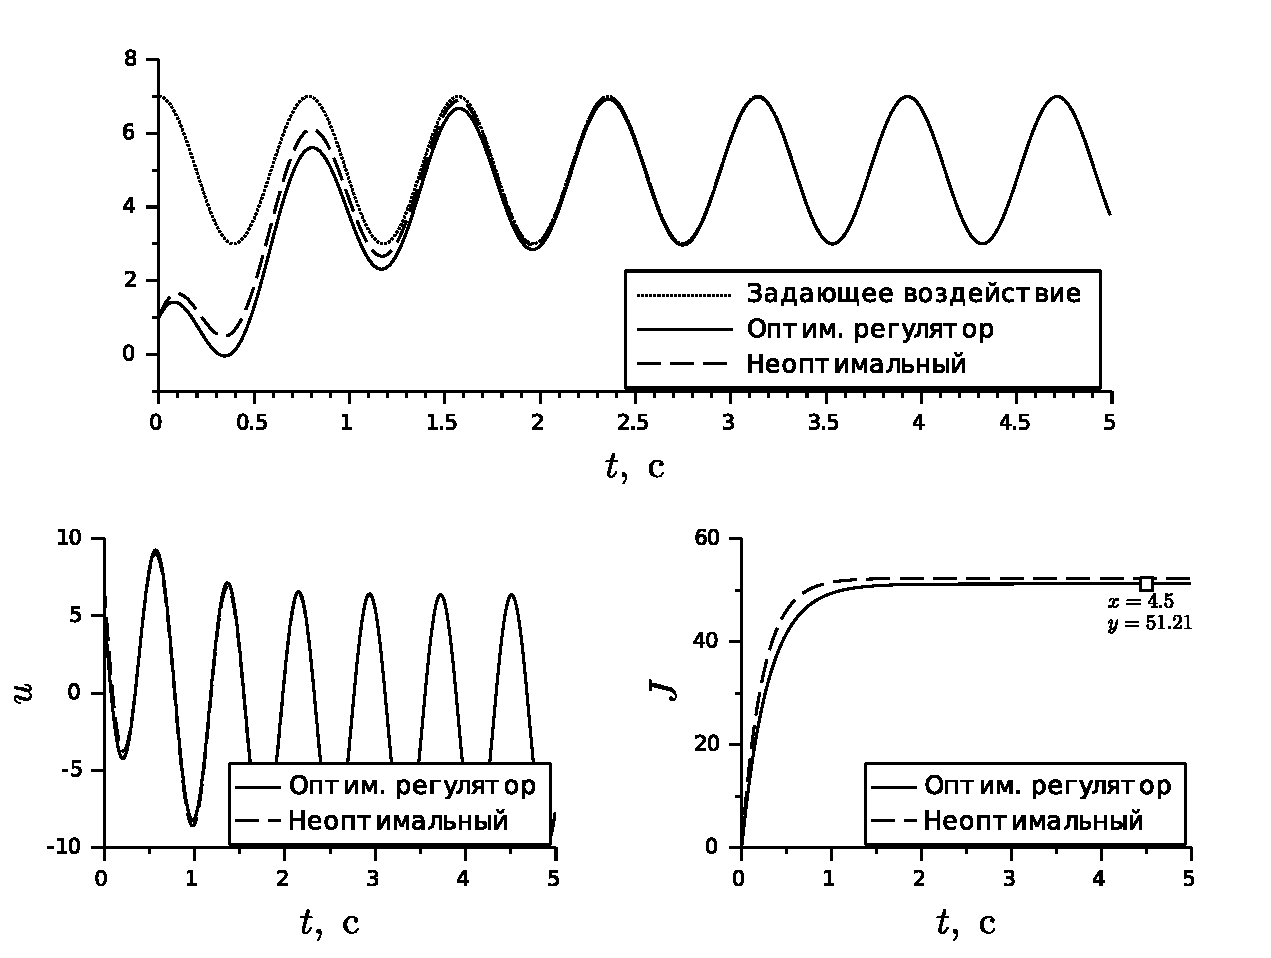
\includegraphics[width=1.0\textwidth]{graphs.pdf}
    \vspace{0cm}
    \caption{Графики переходных процессов в рассматриваемой системе.}
    \label{img_graphs}
\end{figure}


\begin{figure}[h!]
    \centering
    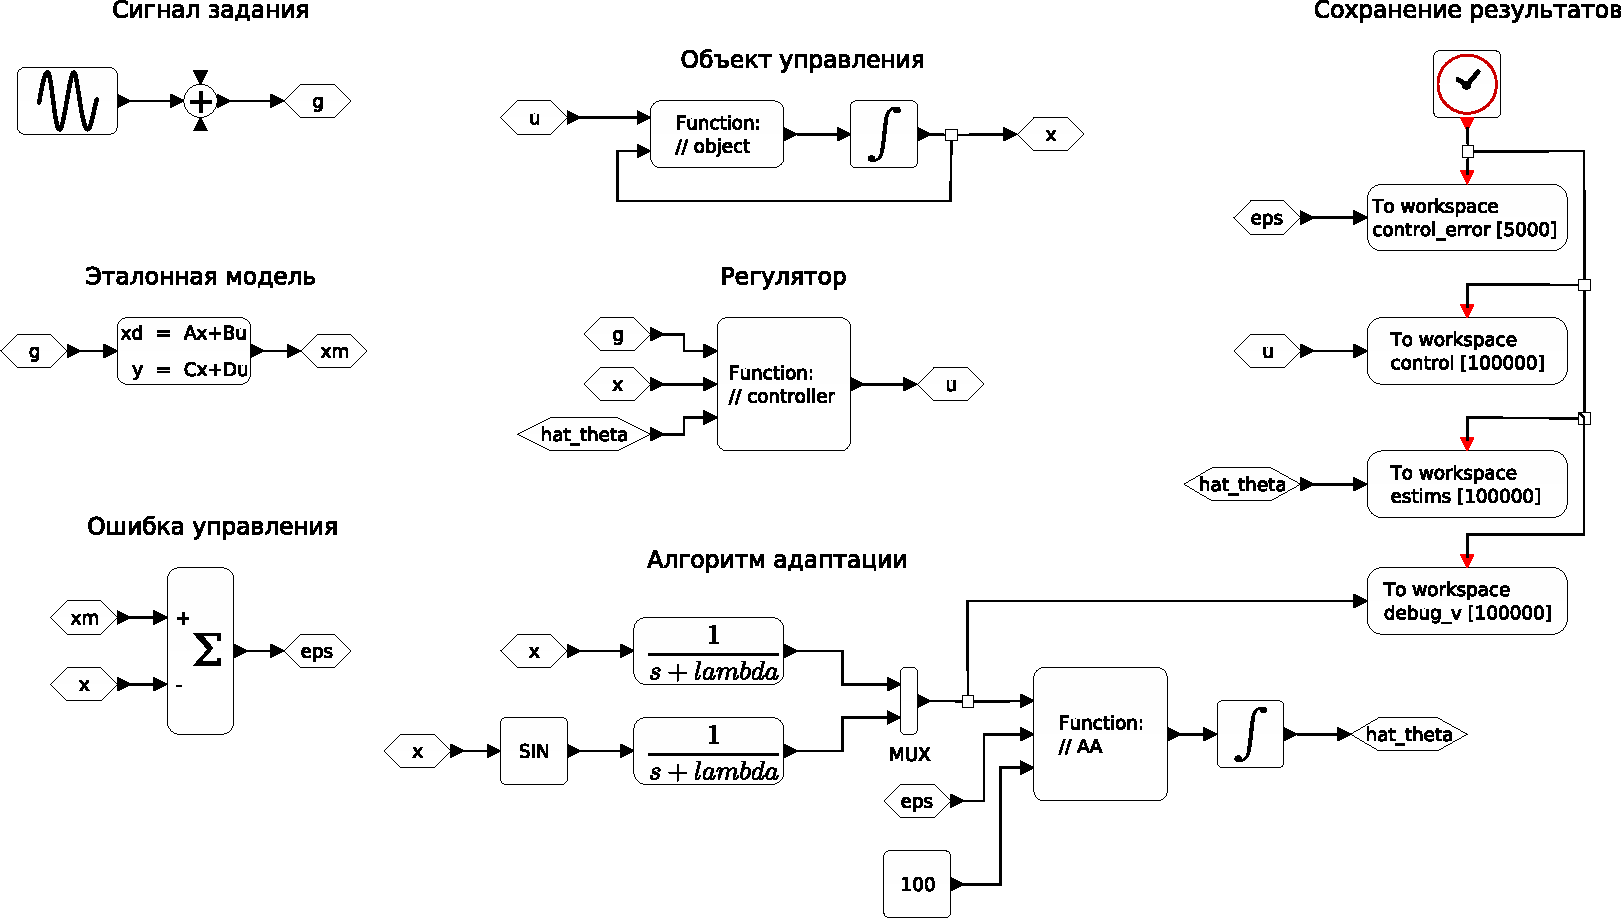
\includegraphics[width=\textwidth]{modeling_scheme.pdf}
    \vspace{0.5cm}
    \caption{Схема моделирования рассматриваемой системы.}
    \label{img_modeling_scheme}
\end{figure}

\newpage
\section{Выводы по работе}
В~результате проделанной работы для заданного ОУ был успешно реализован адаптивный регулятор, минимизирующий заданный критерий качества, характеризующий работу системы и обеспечивающий в установившемся режиме нулевую ошибку слежения переменной состояния ОУ за переменной состояния эталонной модели.
